\section{The downcomer geometry}
\label{sec:geometry}

\subsection{Arrangement}

BOREAS separates the two functions the hairpin conflated. All $\nft$ finned
tubes run downward and exchange heat with the material; a single
\emph{insulated downcomer} returns the whole flow without exchanging. They
meet in a manifold at the bottom of the same borehole.

This is not new construction at depth. A hairpin \emph{is} a bottom
connection --- a U-bend landed at \SI{1500}{\metre} --- and the manifold is
the same class of object: a shop-fabricated assembly run in on the tubing
string, with no cement, no intervention in the formation and no lateral. What
the repurposing inherits is the hole, the casing and the cement, which is
\SIrange{60}{80}{\percent} of a well's cost; everything inside the casing is
new in either geometry.

\begin{figure}[h]
\centering
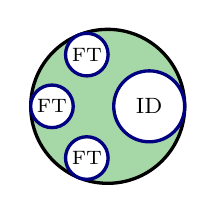
\begin{tikzpicture}[scale=11]
  \fill[green!55!black!35] (0,0) circle (0.0889);
  \draw[very thick] (0,0) circle (0.0889);
  % downcomer, tangent to the wall
  \fill[white] (0.0479,0) circle (0.04096);
  \draw[very thick,blue!50!black] (0.0479,0) circle (0.04096);
  \node at (0.0479,0) {\footnotesize ID};
  % three finned tubes on the opposite side
  \foreach \a in {112,180,248}{
    \fill[white] ({0.0644*cos(\a)},{0.0644*sin(\a)}) circle (0.02458);
    \draw[very thick,blue!50!black] ({0.0644*cos(\a)},{0.0644*sin(\a)})
      circle (0.02458);
    \node at ({0.0644*cos(\a)},{0.0644*sin(\a)}) {\scriptsize FT};}
\end{tikzpicture}
\caption{Borehole cross-section for $\nft = 3$. Shaded: phase-change material,
\SI{60.4}{\percent} of the hole. ID: insulated downcomer,
\SI{82}{\milli\metre} outside diameter, run off-centre. FT: finned tubes over
fins, \SI{49.2}{\milli\metre}. The arrangement is solved rather than sketched;
see Section~\ref{sec:packing}.}
\label{fig:xsec}
\end{figure}

\subsection{Sizing, and why the pressure drop is unchanged}

The downcomer carries the whole flow that the $\nft$ tubes carry between them.
Sizing it for equal velocity therefore means equal total area,
\begin{equation}
\pi\rid^{2} = \nft\,\pi r_i^{2}
\qquad\Longrightarrow\qquad
\rid = r_i\sqrt{\nft}\,,
\label{eq:ridsize}
\end{equation}
giving \SI{28.1}{\milli\metre} for three \SI{1.25}{inch} Sch.\,80 tubes.

The consequence is worth stating carefully, because it is the reason this
geometry was chosen over the alternatives. Let the total well flow be $\md$.
In the hairpin, the flow divides among $n$ hairpins, each a serial path of
area $\pi r_i^2$ and length $2\Lw$, so the velocity is
$u_h = \md/(n\rho\pi r_i^{2})$. In BOREAS, the flow divides among $\nft$ tubes
of the same area over length $\Lw$, and then passes through the downcomer of
area $\nft \pi r_i^2$ over length $\Lw$; by~\eqref{eq:ridsize} the velocity in
both is $u_b = \md/(\nft\rho\pi r_i^{2})$. With $n = \nft$ the velocities are
equal and the total developed length is $2\Lw$ in both cases, so to the extent
that friction factors agree, \emph{the pressure drop is identical}.

This matters because the v0.16 parametric study established that the entire
below-ground influence on round-trip efficiency is pumping: regressing
$\etarte$ on the pumping fraction $f_{\mathrm{pump}}$ alone gives
$R^2 = 0.956$, and within the low-pumping block $\etarte$ varies by less than
one percent. A geometry change that cost pumping would be charged directly
against the only quantity that was moving. The nested-coaxial alternative, in
which the return runs inside each finned tube, preserves storage volume
equally well but divides each bore into two passages plus insulation, leaving
\SI{5.27}{\centi\metre\squared} of each against \SI{19.05}{\centi\metre\squared}
undivided --- a velocity ratio of 1.81 and a pressure-drop factor of 3.3.

\subsection{Packing}
\label{sec:packing}

The downcomer is run off-centre. A concentric arrangement requires
$r_{\mathrm{id},o} + 2(r_e + L_{\mathrm{fin}}) \le R_c$, which for three
\SI{1.25}{inch} tubes in a \SI{7}{inch} hole fails by about
\SI{1}{\milli\metre}. Placing the downcomer tangent to the casing and
distributing the finned tubes on the opposite arc, both tangent circles of
radii $d_{\mathrm{id}} = R_c - r_{\mathrm{id},o}$ and
$d_{\mathrm{ft}} = R_c - (r_e + L_{\mathrm{fin}})$, the smallest angular
offset that clears the downcomer follows from the cosine rule,
\begin{equation}
\cos\theta_{\min} = \frac{d_{\mathrm{id}}^{2} + d_{\mathrm{ft}}^{2}
  - (r_e + L_{\mathrm{fin}} + r_{\mathrm{id},o})^{2}}
  {2\,d_{\mathrm{id}}\,d_{\mathrm{ft}}},
\end{equation}
and the tubes are spread over the remaining $2\pi - 2\theta_{\min}$. This
closes with clearance for $\nft \le 5$; six \SI{1.25}{inch} tubes plus the
downcomer overlap by \SI{12}{\milli\metre} and do not fit. The check is
performed in code and reported beneath the figure, because a schematic that
nobody verifies is a drawing rather than a result.

\subsection{Storage volume and cell radius}

The downcomer occupies cross-section but exchanges no heat with the material
it displaces, so it is subtracted before the cells are formed rather than
counted as a participant:
\begin{equation}
V_{\mathrm{pcm}} = \Lw\Big[\pi R_c^{2}
  - \nft\big(\pi r_e^{2} + n_{\mathrm{fin}} t_{\mathrm{fin}} L_{\mathrm{fin}}\big)
  - \pi r_{\mathrm{id},o}^{2}\Big],
\qquad
\pi r_c^{2} = \frac{\pi\big(R_c^{2} - r_{\mathrm{id},o}^{2}\big)}{\nft}.
\end{equation}
At the default geometry this gives \SI{22.85}{\metre\cubed} of material per
borehole, \SI{60.4}{\percent} of the hole, and $r_c = \SI{45.6}{\milli\metre}$
against a casing radius of \SI{88.9}{\milli\metre}. The cell radius is the
radius at which a tube's melt front meets its neighbour's, and it is not the
borehole wall: a merge limit imposed at the wall would be a factor of two too
permissive and therefore silent at every design point.

\subsection{The downcomer bypass leak}
\label{sec:bypass}

The downcomer is insulated but not adiabatic. Its resistance per unit length
is $R_{\mathrm{ins}} = \ln(r_{\mathrm{id},o}/\rid)/2\pi k_{\mathrm{ins}}
= \SI{8.56}{\metre\kelvin\per\watt}$, two orders above the formation path, so
the two mechanisms do not compete; they are nonetheless reported separately,
because they have different signs and different meanings.

\paragraph{The sign reverses between half-cycles, and the two are not equal.}
On charge the downcomer carries the \SI{160}{\degC} supply \emph{down} past
material grading \SI{101}{\degC} at the top to \SI{150}{\degC} at the bottom,
so heat leaks out of the pipe and into the store. The energy is not lost: it
is deposited in the wrong layer, at a large temperature mismatch. This is an
exergy penalty rather than an energy one, and it is an advantage of this
geometry over the nested coaxial, where the insulated passage carries the
\emph{cold} return and its leak un-stores heat and returns it to the heat
pump. On discharge the downcomer carries the hot outlet back up past the same
material and re-deposits heat just extracted, which is a true capacity loss,
and the larger of the two because the driving difference is larger.

